% Authors: Greg Westphal and Kathryn Huff
\documentclass[border=10pt]{standalone}
\usepackage{tikz}
\usetikzlibrary{arrows.meta}
\tikzset{%
  >={Latex[width=2mm,length=2mm]},
  % Specifications for style of nodes:
            base/.style = {rectangle, rounded corners, draw=black,
                           minimum width=3cm, minimum height=1cm,
                           text centered, font=\sffamily},
       bluebox/.style = {base, fill=gray!15}, %blue!30
       redbox/.style = {base, fill=white!30}, %red
       greenbox/.style = {base, fill=white!30}, %green
       process/.style = {base, minimum width=2.5cm, fill=gray!30, %orange!15
                           font=\ttfamily},
}
% Drawing part, node distance is 1.5 cm and every node
% is prefilled with white background
\begin{document}
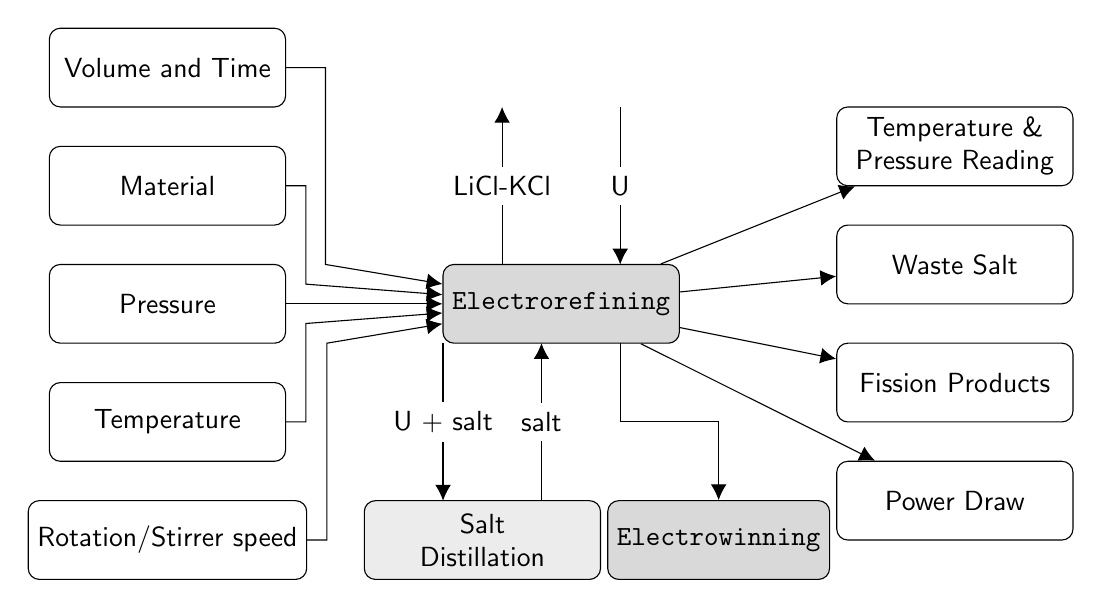
\begin{tikzpicture}[node distance=3cm,
    every node/.style={fill=white, font=\sffamily}, align=center]
  % Specification of nodes (position, etc.)
  
 
  \node (refining)			[process] {Electrorefining};
  \node (winning)			[process, below of=refining, xshift=2cm] {Electrowinning};
  \node (temp)	 			[greenbox, left of=refining, xshift=-2cm, yshift=-1.5cm] {Temperature};
  \node (fission) 			[redbox, right of=refining, xshift=2cm, yshift=-1cm] {Fission Products};
  \node (pressure)			[greenbox, left of=refining, xshift=-2cm] {Pressure};
  \node (rotation)	 		[greenbox, left of=refining, xshift=-2cm, yshift=-3cm] {Rotation/Stirrer speed};
  \node (material)			[greenbox, left of=refining, xshift=-2cm, yshift=1.5cm] {Material};
  \node (vol)				[greenbox, left of=refining, xshift=-2cm, yshift=3cm] {Volume and Time};
  \node (power)				[redbox, right of=refining, xshift=2cm, yshift=-2.5cm] {Power Draw};
  \node (waste)				[redbox, right of=refining, xshift=2cm, yshift=0.5cm] {Waste Salt};
  \node (temp+press)		[redbox, right of=refining, xshift=2cm, yshift=2cm] {Temperature \& \\ Pressure Reading};
  
  \node (salt distl)		[bluebox, below of=refining, xshift=-1cm] {Salt \\ Distillation};
  
  
  \draw[->]					(material.east) -- ++(0.25,0) --++(0,-1.25) -- (refining);;
  \draw[->]					(refining) -- (temp+press);
  \draw[->]					(refining) -- (waste);
  \draw[->]					(refining) -- (power);
  \draw[->]					(pressure) -- (refining);
  \draw[->]					(temp.east) -- ++(0.25,0) --++(0,1.25) -- (refining);
  \draw[->]					(rotation.east) -- ++(0.25,0) --++(0,2.5) -- (refining);
  \draw[->]					(refining) -- (fission);
  \draw[->]					(vol.east) -- ++(0.5,0) --++(0,-2.5) -- (refining);
  
  \draw[->]					(refining)++(0.75,-0.5) -- ++(0,-1) -- ++(0.75,0) -| (winning);
  \draw[->]					(refining)++(-1.5,-0.5) -- ++(0,-2)(salt distl) node[midway] {U + salt};
  \draw[->]					(salt distl)++(0.75,0.5) -- ++(0,2) (refining) node[midway] {salt};
  \draw[->]					(refining)++(0.75,2.5) -- ++(0,-2) node[midway] {U};
  \draw[->]					(refining)++(-0.75,0.5) -- ++(0,2)  node[midway] {LiCl-KCl};

  \end{tikzpicture}
\end{document}